\documentclass[oneside,ti]{iiufrgs}
% um tipo específico de monografia pode ser informado como parâmetro opcional:
%\documentclass[tese]{iiufrgs}
% monografias em inglês devem receber o parâmetro `english':
%\documentclass[diss,english]{iiufrgs}
% a opção `openright' pode ser usada para forçar inícios de capítulos
% em páginas ímpares
% \documentclass[openright]{iiufrgs}
% para gerar uma versão somente-frente, basta utilizar a opção `oneside':
% \documentclass[oneside]{iiufrgs}
\usepackage[T1]{fontenc}        % pacote para conj. de caracteres correto
\usepackage[utf8]{inputenc}	    % pacote para acentuação
\usepackage[alf]{abntcite}		% pacote para as referencias da abnt nao numerica
\usepackage{graphicx}           % pacote para importar figuras
\usepackage{times}              % pacote para usar fonte Adobe Times
\usepackage{color}              % pacote para usar \textcolor
\usepackage{listings}       	% pacote para usar listagens/listing
\usepackage{rotating}		   	% pacote para rotacoes
\usepackage{xcolor,colortbl}	% colorir tabelas
%\usepackage{mathptmx}          % p/ usar fonte Adobe Times nas fórmulas
%\usepackage{setspace}			% p/ usar singlespacing
\usepackage{wrapfig}			% p/ usar figuras em volta do texto...

% Use todo para anotar algo para ver depois
% Criando comando \todo{algo}
\newcommand{\todo}[1] {\footnote{TODO #1}\marginpar{\textcolor{red}{\textbf{TODO}}}}
%\newcommand{\todo}[1] {}
% Use dev para anotar algum comprometimento
\newcommand{\dev}[1] {\marginpar{\textcolor{blue}{\textbf{IMPL}}}}
%\newcommand{\dev}[1] {}

% Traduzindo Listing
\renewcommand{\lstlistingname}{Listagem}
\renewcommand{\lstlistlistingname}{Lista de Listagens}

%
% Informações gerais
%
\title{Jason com serviços Web:\\agentes e ambientes heterogêneos}

\author{Lucca}{Ricardo Rodrigues}
% alguns documentos podem ter varios autores:
%\author{Flaumann}{Frida Gutenberg}
%\author{Flaumann}{Klaus Gutenberg}

% orientador e co-orientador são opcionais (não diga isso pra eles :))
\advisor[Prof.~Dr.]{Bordini}{Rafael Heitor}
%\coadvisor[Prof.~Dr.]{Meu}{Seila Ainda}

% a data deve ser a da defesa; se nao especificada, são gerados
% mes e ano correntes
%\date{maio}{2001}

% o nome do curso pode ser redefinido (ex. para TCs)
%\course{Curso de Especialização em Cachaça}

% o local de realização do trabalho pode ser especificado (ex. para TCs)
% com o comando \location:
%\location{Itaquaquecetuba}{SP}

% itens individuais da nominata podem ser redefinidos com os comandos
% abaixo:
% \renewcommand{\nominataReit}{Prof\textsuperscript{a}.~Wrana Maria Panizzi}
% \renewcommand{\nominataReitname}{Reitora}
% \renewcommand{\nominataPRE}{Prof.~Jos{\'e} Carlos Ferraz Hennemann}
% \renewcommand{\nominataPREname}{Pr{\'o}-Reitor de Ensino}
% \renewcommand{\nominataPRAPG}{Prof\textsuperscript{a}.~Joc{\'e}lia Grazia}
% \renewcommand{\nominataPRAPGname}{Pr{\'o}-Reitora Adjunta de P{\'o}s-Gradua{\c{c}}{\~a}o}
% \renewcommand{\nominataDir}{Prof.~Philippe Olivier Alexandre Navaux}
% \renewcommand{\nominataDirname}{Diretor do Instituto de Inform{\'a}tica}
% \renewcommand{\nominataCoord}{Prof.~Carlos Alberto Heuser}
% \renewcommand{\nominataCoordname}{Coordenador do PPGC}
% \renewcommand{\nominataBibchefe}{Beatriz Regina Bastos Haro}
% \renewcommand{\nominataBibchefename}{Bibliotec{\'a}ria-chefe do Instituto de Inform{\'a}tica}
% \renewcommand{\nominataChefeINA}{Prof.~Jos{\'e} Valdeni de Lima}
% \renewcommand{\nominataChefeINAname}{Chefe do \deptINA}
% \renewcommand{\nominataChefeINT}{Prof.~Leila Ribeiro}
% \renewcommand{\nominataChefeINTname}{Chefe do \deptINT}

% A seguir são apresentados comandos específicos para alguns
% tipos de documentos.

% Relatório de Pesquisa [rp]:
% \rp{123}             % numero do rp
% \financ{CNPq, CAPES} % orgaos financiadores

% Trabalho Individual [ti]:
 \ti{123}     % numero do TI
% \ti[II]{456} % no caso de ser o segundo TI

% Trabalho de Conclusão [tc]:
% além de definir explicitamente o nome do curso (\course) e o local
% de realização (\location), é necessário redefinir a nominata,
% pois as informações necessárias dependem do curso. Ex.:
%\renewcommand{\nominata}{
%        UNIVERSIDADE FEDERAL DO RIO GRANDE DO SUL\\
%        Reitora: Prof\textsuperscript{a}.~Wrana Maria Panizzi\\
%        Pró-Reitor de Ensino: Prof.~José Carlos Ferraz Hennemann\\
%        Diretor do Instituto de Informática: Prof.~Philippe Olivier Alexandre Navaux\\
%        Coordenador do curso: Prof.~Seu Creysson\\
%        Bibliotecária-chefe do Instituto de Informática: Beatriz Regina Bastos Haro
%}

% Monografias de Especialização [espec]:
% \espec{Redes e Sistemas Distribuídos}      % nome do curso
% \coord[Profa.~Dra.]{Weber}{Taisy da Silva} % coordenador do curso
% \dept{INA}                                 % departamento relacionado

%
% palavras-chave
% iniciar todas com letras minúsculas, exceto no caso de abreviaturas
%
\keyword{sistemas multi-agente}
\keyword{agentes cognitivos}
\keyword{serviços web}
\keyword{XML-RPC}

%
% inicio do documento
%
\begin{document}

% folha de rosto
% às vezes é necessário redefinir algum comando logo antes de produzir
% a folha de rosto:
% \renewcommand{\coordname}{Coordenadora do Curso}
\maketitle

%% dedicatoria
\clearpage
\begin{flushright}
\mbox{}\vfill
{\sffamily\itshape
``If I have seen farther than others,\\
it is because I stood on the shoulders of giants.''\\}
--- \textsc{Sir~Isaac Newton}
\end{flushright}

%% agradecimentos
\chapter*{Agradecimentos}
Agradeço ao \LaTeX\ por não ter vírus de macro\ldots


\tableofcontents % sumario

% lista de abreviaturas e siglas
% o parametro deve ser a abreviatura mais longa
\begin{listofabbrv}{IHC}
		\item[AOP] \underline{A}gent \underline{O}riented \underline{P}rogramming
		\item[ASL] \underline{A}gent\underline{S}peak \underline{L}anguage
		\item[BDI] \underline{B}elief-\underline{D}esire-\underline{I}ntention
        \item[IHC] \underline{I}ntera\c{c}\~{a}o \underline{H}omem-\underline{C}omputador
        \item[OCC] \underline{O}rtony \underline{C}lore e \underline{C}ollins
		\item[OWL] \underline{O}ntology \underline{W}eb \underline{L}anguage
		\item[UEM] \underline{U}rban \underline{E}nvironment \underline{M}odel
        \item[UML] \underline{U}nified \underline{M}odeling \underline{L}anguage
        \item[XML] e\underline{X}tensible \underline{M}arkup \underline{L}anguage

\end{listofabbrv}



\listoffigures % lista de figuras, se houver mais de 3
%\listoftables % lista de tabelas, se houver mais de 3
\lstlistoflistings % lista de listagens, se houver mais de 3
\definecolor{darkgray}{rgb}{0.95,0.95,0.95}
\lstset{backgroundcolor=\color{darkgray}}
\lstset{numbers=left, basicstyle=\scriptsize\ttfamily, numberstyle=\tiny, stepnumber=2, numbersep=5pt}

% resumo na língua do documento
\begin{abstract}
Este trabalho apresenta um \emph{framework} que permite aos agentes perceberem
suas próprias emoções. Ele foi feito em \emph{Java} e usa a plataforma
multi-agente \emph{Jason}, sendo que estende a base de crenças da última a fim
de utilizar à ontologia afetiva desenvolvida. Além disso, o ambiente foi
construído a partir de uma base de conhecimento que descreve rotinas.
Adicionalmente, um mecanismo de avaliação das emoções baseando-se nas anotações dos
objetos foi construído apoiado por uma ontologia de preferência sobre essas
anotações. Dessa forma, aplicações de entretenimento poderiam utilizar o
sistema ou as bases de conhecimento apresentadas para diferentes propósitos. A criação de
um mapa onde os personagens atuam, a criação da rotina de cada personagem e
suas preferências são alguns exemplos de utilizações. Para validação desse
desenvolvimento, dois exemplos foram construídos. O primeiro exemplo com a
finalidade principal de demonstrar que o modelo afetivo atingiu a maior parte
dos grafos afetivos. Enquanto, o segundo usa apenas grupo emotivo e serve para
demonstrar a utilização conjunta de todas as ontologias apresentadas.
\end{abstract}

%Example:
%http://www.sbgames.org/sbgames2011/proceedings/sbgames/papers/comp/full/11-92076_2.pdf
%1º, o que é o trabalho
%2º, o que uso e para que
%3º, para que posso utiliza-la
%4º, foi falado que um experimento para validar a arquitetura foi criado

% resumo na outra língua
% como parametros devem ser passados o titulo e as palavras-chave
% na outra língua, separadas por vírgulas
%\begin{englishabstract}{Maro: An emotional model using ontology}{virtual
%agents, programming, agents, simulation, affective computing, OCC's model, ontology}
%This work presents a framework built to work with Jason's platform
%\cite{bordini-jason} to allow agents acknowledge their own emotions. This work have
%been developed in \emph{Java} and extended the belief base from agent of
%platform to utilize an developed ontology based on the affective model
%\cite{ortony1988cse}. For so the development of a belief base permits an agent
%perceive emotions based on your appraisal of environment and conclude new
%beliefs. In addition, an ontology to make the schedules of agents and to make
%yours preferences about annotations on belief were developed. So,
%entertainment applications and games could use the three ontologies together
%to create a map of the city, to create schedules or routines of each
%agent and to give preferences about annotations used in beliefs that came from
%environment. Finally, to validate the framework has been developed an
%soccer's application to demonstrate many emotions from affective model.
%\end{englishabstract}
 % inclui o resumo da lingua nativa e estrangeira

% aqui comeca o texto propriamente dito
\chapter{Introdução}

Ontologia foi caracterizada como o estudo da existência, desde Aristóteles,
por estar interessada em descrever todas as coisas existentes e as relações
que existem entre elas. Atualmente, essa forma de representar o domínio do
conhecimento tem se tornado popular na computação por causa da independência
de sistema oferecida.

Segundo \citet{gruber1993translation}, uma ontologia é uma especificação explícita do
domínio sendo tratado. Além disso, ele aplica esse conceito em sistemas
baseados em conhecimento onde o domínio é representado por um formalismo
declarativo e o conjunto de conceitos e relações forma o vocabulário usado
pelo sistema. Esse vocabulário provém um conjunto de termos bem formados para
o sistema trabalhar.
%
Entretanto \citet{ontoly2004Approach}, definiu ontologia como uma representação
do conhecimento usado para capturar outras informações ou conhecimentos sobre
o assunto. Atualmente, ontologias são vistas como um entendimento comum e
compartilhado de um domínio que pode ser utilizado na comunicação entre
máquinas ou entre pessoas \cite{wks2008towards}.

O presente trabalho foi baseado na linguagem OWL (\emph{Ontology Web
Language}). Essa linguagem foi regulamentada pela W3C\footnote{Ver
\url{http://www.w3.org/standards/semanticweb/ontology}.}, orgão internacional
que regulamenta padrões na Web, para ser usada na \emph{Web} Semântica.
Essa linguagem foi criada em 2002 com o proposito de criação de ontologias e
trabalha com a hipótese de mundo aberto, isto é, nada é afirmado por não ser
dito. Infelizmente, para a W3C não há uma distinção clara entre vocabulário e
ontologia.

A linguagem OWL permite a especificação de conceitos e não de suas instâncias.
Sendo assim, não é possivel descrever uma regra simples como um conceito de
igualdade onde duas relações distintas tem que chegar na mesma instância
final. %Outro exemplo, o conceito de tios que são os irmãos de meus pais não é
%possível ser feita na OWL. A versão 2 da OWL permite a descrição do conceito
%de tios, porém o conceito de igualdade permanece impossível.
%
A linguagem SWRL (\emph{Semantic Web Rule
Language})\footnote{Mais detalhes \url{http://www.w3.org/Submission/SWRL/}.}
recomendada pela W3C permite escrever regras lógicas que melhoram a
precisão dos conceitos sendo descritos porque permite lidar com as suas
instâncias. Dessa forma, a SWRL supri uma falta até então não tratada pela
linguagem OWL e, por isso, seu uso em conjunto é extremamente poderoso. Essas
duas linguagens juntas permitem a escrita do conceito de igualdade descrito
anteriormente.

A ferramenta \emph{Protege}\footnote{Mais informações, consulte \url{http://protege.stanford.edu}.}
em sua versão 4.1 suporta a linguagem OWL 2 juntamente com a SWRL. Ha suporte
aos raciocinadores chamados \emph{FaCT++}, \emph{HermiT} e \emph{Pellet}.
O raciocinador é uma peça importante porque é através dele que a ontologia
será questionada, isto é, somente com um raciocinador ativo é possível saber
se uma instância pertence a determinado conceito. O raciocinador
\emph{Pellet}\dev{} é o que esta sendo utilizado pelo presente autor por
seu excelente suporte a explicações de inconsistência.

A área da computação que estuda as emoções é denominada Computação Afetiva por
\citet{Pic98}. As emoções, segundo \citet{damasio2004erro}, podem ser divididas
entre primárias (não-cognitivas) e secundárias (cognitivas). As emoções
primárias surgem a partir de reações a determinados estímulos e são geradas
rapidamente. Já as emoções secundárias são aprendidas ao longo da nossa vida,
isto é, são geradas por uma avaliação de uma situação de acordo com nossos
objetivos e valores morais. Entretanto, essa divisão ainda não esta
consolidada porque o fato de haver menos atividade cognitiva não quer dizer
que esta atividade não exista.

\citet{bates1994role} foi um dos primeiros a trabalhar na utilização de
emoções na área de animação. Nessa área, o estudo do comportamento humano é
realizado visando realizar a imitação das ações humanas. Assim, simulando
essas atitudes de uma pessoa de tal maneira que pareça possuir vida própria.
Seu trabalho utilizou o modelo de emoções proposto por \citet{ortony1988cse}.
Esse modelo fundamenta ao todo 22 emoções diferentes divididos em três
formas de percepção: ações, eventos e objetos.

%\begin{figure*}
%  \centering
%    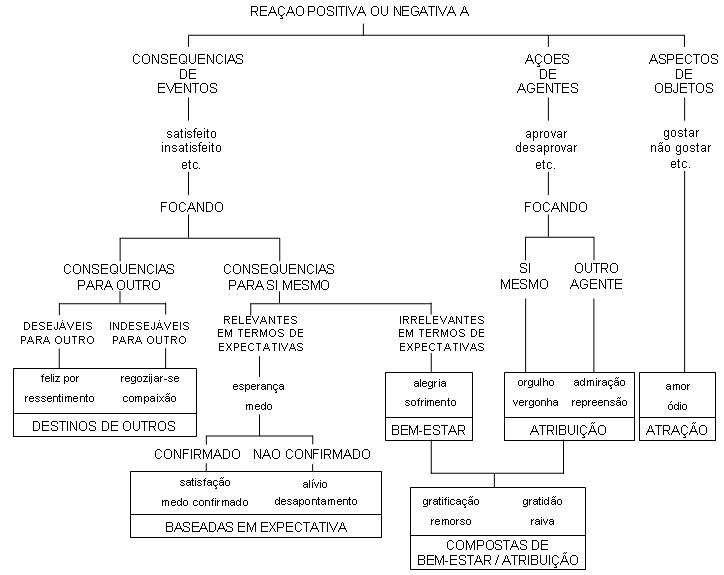
\includegraphics[width=100mm]{figuras/pontarolo_occ.png}
%  \caption{Modelo OCC adaptado de \cite{pontarolo2008modelagem}.}
%  \label{fig:occ_model_original}
%\end{figure*}

A Figura~X\footnote{removido por agora} mostra uma visualização da estrutura
lógica das emoções. As emoções no modelo de \citet{ortony1988cse} já
encontram-se agrupadas em grupos por estarem utilizando regras semelhantes ou
próximas. Esses grupos são representados pelo quadrados e nome do grupo é dado
na parte inferior, assim o ramo de objetos que julga a atração de um indivíduo
com alguma outra coisa (agente ou objeto) possui o grupo de Atração. O ramo de
ações julga a responsabilidade de um agente sobre suas ações e o ramo de
eventos julga a consequência de eventos ou ações desempenhadas. Desse ramo,
o grupo Destinos de outros julga sempre algum outro agente que não é aquele
que esta fazendo a avaliação. Além disso, o grupo denominado Compostas de
Bem-Estar/Atribuição junta os grupos de Bem-Estar (consequência de um evento
sem expectativa) com Atribuição (responsabilidade).

O presente trabalho pretende estudar diferentes ontologias do modelo afetivo
\cite{benta2007ontology,wks2008towards,springerlink:10.1007/978-3-642-01639-448,lera2009semantic}
visando o entendimento destas e suas diferenças. Entretanto, nenhum trabalho propôs
a junção de uma ontologia afetiva com uma humanos virtuais
\cite{Rojas:2006:IRM:1174429.1174442,Gutierrez:2007:OVH:1229160.1229164} com
uma que explique como tratar as percepções do ambiente.


%\chapter{Metodologia}

\section{Atividades previstas}

\begin{enumerate}
	\item Estudo bibliográfico sobre as estratégias existentes de integração de softwares;
	\item Elaboração da proposta de TI e escolha de um segundo orientador (em atendimento à regra do PPGC);
	\item Desenvolvimento da estratégia definida no Jason;
	\item Validação da solução através de ambientes e agentes desenvolvidos em Python;
	\item Redação da monografia;
\end{enumerate}

\section{Cronograma das atividades}

	\begin{tabular}[c]{c|cccccc}
		Atividades & \begin{sideways} \small{Jul/10} \end{sideways}& \begin{sideways} \small{Ag/10} \end{sideways}& \begin{sideways} \small{S/10} \end{sideways}& \begin{sideways} \small{O/10} \end{sideways}& \begin{sideways} \small{N/10} \end{sideways}& \begin{sideways} \small{D/10} \end{sideways} \\ \hline
		%\cellcolor{gray!50} pendente & \\
		%\cellcolor{green!50} feito & \\
		%\cellcolor{blue!50} andamento & \\
		%\cellcolor{red!85} atrasado &  \\
	Estudo bibliográfico & \cellcolor{gray!50} & \cellcolor{gray!50} & \cellcolor{gray!50} &  &  &  \\
	Elaboração proposta &  & \cellcolor{gray!50} &  &  &  &  \\
	Desenvolvimento da estratégia &  &  & \cellcolor{gray!50} &  &  &  \\
	Validação da solução &  & & \cellcolor{gray!50} & \cellcolor{gray!50} &  &   \\
	Redação da monografia &  & \cellcolor{gray!50} & \cellcolor{gray!50} & \cellcolor{gray!50} & \cellcolor{gray!50} &
	\end{tabular}

% Veja modelo em https://saloon.inf.ufrgs.br/twiki-data/PEP/PepEder/pep_v4.pdf

\chapter{Estado da Arte}

\todo{rever}
%A presente seção se encontra divida em uma introdução a programação de
%agentes na seção~\ref{AOP}, onde é discutido o paradigma e os termos agentes
%e personagens. Na seção~\ref{CA:1} a área de computação afetiva é
%apresentada.  O conceito de ontologia é debatido na seção~\ref{onto} e os
%trabalhos relacionados são apresentados na seção~\ref{TR}.

\section{Conceitos de Agente}

\citet{laird2001human} afirmam que a pesquisa em Inteligência Artificial tem
sido fragmentada em muitas áreas especializadas e, assim, algoritmos
específicos e mais eficientes podem ser criados.
%
Há várias definições do conceito de Agente, por exemplo
\cite{shoham1993agent,roadmap,fatemeh2009multi}. \citet{shoham1993agent}
propõe que Agente é uma entidade definida por componentes mentais como
crenças, habilidades, escolhas e comprometimentos.

\citet{franklin1997agent} define um agente através das características que a
entidade deve apresentar.  Atualmente, o menor conjunto comumente aceito
dessas características é composto por três conceitos principais: (i)
Autonomia; (ii) Sociabilidade; (iii) Situacionalidade.
\citet{roadmap,fatemeh2009multi} concordam que autonomia é quando um Agente
toma suas próprias decisões independente de qualquer outra entidade do sistema
ou, ainda, da intervenção diretas de seres humanos. A característica de
sociabilidade permite flexibilidade na execução das tarefas, através da
interação com outros agentes que estejam presentes no sistema. A última,
permite que o agente situe-se em um ambiente dinâmico interagindo com o mesmo
através de algum tipo de sensor ou atuador.

\citet{ingrand1992architecture} indicam que entidades autônomas podem ter a
capacidade de expor seus dados internos para que seja possível um usuário,
possivelmente humano, dar dicas sobre a forma de resolução dos problemas sendo
enfrentados. Esta visão não conflita com a noção de autonomia exposta acima,
pois o agente permanece independente para tomar suas decisões podendo rejeitar
as dicas ou sugestões enviadas pelo usuário.

\citeauthor{ingrand1992architecture} também define Agente em um ambiente com
componentes heterogêneos e com diferentes tempos de resposta para a execução
de suas tarefas. \citet{doyle1998annotated} estendem o conceito dizendo que os
objetos pertencentes ao ambiente devem conter anotações que determinam a forma
de uso dos objetos disponibilizados neles. Assim, não se sabe como todos os
objetos funcionam e, sim, uma forma de aprender com o próprio objeto a sua
forma de utilização. \citet{shoham1993agent} define sociabilidade como uma
habilidade cognitiva necessária para o desempenho das suas tarefas.

Essas inúmeras definições do termo Agente não permite saber se ele é um ser
físico ou abstrato. Dessa forma, \citet{nareyek2001review,damiano2008emotions}
defendem que o agente é o ser abstrato de um ator físico. Em outras palavras,
o ser que age ou atua no meio é chamado de personagem ou ator. Enquanto a
mente desse ser é chamada de agente.

\section{Paradigma de Programação Orientada a Agentes}

\citet{shoham1993agent} propôs em seu trabalho a linguagem \emph{Agent-0} uma
das primeiras a serem baseadas em atos de fala e uma nova visão para se
programar.  Esses atos de fala podem ser vistos como comandos falados entre
atores com as mais diversas finalidades (informar, perguntar, requerer,
aceitar, etc).  Dessa forma, \citeauthor{shoham1993agent} tentou promover a
idéia de computação com uma interação mais social entre membros de um sistema.
Em outras palavras, esse novo paradigma de programação precisa que exista
cooperação e competição entre os agentes para a realização das tarefas
desejadas.

Assim, o agente encontra-se situado em um ambiente no qual pode receber
informações de outros agentes, assim como enviar para outros.  As ações são
estabelecidas utilizando regras que descrevem comportamentos. Assim, é
possível, a própria entidade decidir qual ação deve ser tomada. Essas regras
são construídas em fórmulas lógicas descrevendo-se o contexto que torna um
curso de ação válida e sua consequência que é o conjunto de ações a serem
desempenhadas.

Atualmente, há diversas linguagens para a programação de agentes, por exemplo:
\emph{2APL}, \emph{Agent-0}, \emph{AgentSpeak(L)}, \emph{GOAL} e
\emph{MetateM}~\cite{bordini2009multi}. Elas são baseadas em diversos
formalismos diferentes. MetateM por exemplo é baseada em lógica temporal,
permitindo que formulas temporais definindo o comportamento do agente sejam
diretamente executadas.

A plataforma \jason \cite{bordini-jason} utilizada no trabalho pode ser
pensada como um sistema de planejamento reativo, em que planos são executados
a partir de alterações nas crenças e objetivos do agente. A plataforma
baseia-se na arquitetura BDI e utiliza uma extensão da linguagem de
programação abstrata, definida por \citet{rao1996agentspeak}, chamada
AgentSpeak(L), para especificar o reciocínio sobre ações dos agentes. A grande
vantagem dessa plataforma é a rapidez com que melhorias têm sido feitas e a
facilidade de customização de diversos componentes da plataforma.

\section{Computação Afetiva}

\citet{Pic98} definiu Computação Afetiva como uma ``computação relacionada,
surgida ou que influência as emoções''. Além disso, computadores com emoções
permitem aos mesmos um determinado nível de comportamento inteligente e
criatividade que seria impossível sem as emoções e esse é o principal desafio
dessa área. Logo, o seu entendimento pode explicar fenômenos como, por
exemplo, atenção, memória e outros.


Essa área é normalmente dividida em duas sub-áreas. A primeira estuda o
reconhecimento e a expressão de emoções dentro da Interação Homem-Computador;
a segunda, foca na síntese de emoções para aprimorar os seres robóticos e/ou
para estudar o comportamento humano por meio de simulações. Há muita
aplicabilidade dessas técnicas, por exemplo: a área que reconhece as emoções
pode ser utilizada para adaptar o sistema ao estado da pessoa permitindo ao
mesmo instruí-la, questioná-la, encorajá-la ou ocultar determinadas
informações consideradas irrelevantes.

O objetivo de \citet{bick2003relational} com o projeto \emph{Relational
Agents} é possibilitar aos usuários a criação de um relacionamento social e
emocional com longa duração.  Em \citet{bickmore2009virtual}, a confiança no
agente torna possível discutir tarefas mais importantes como melhoria da saúde
ou até a compra de uma casa. Outro trabalho na área de IHC é o reconhecimento
de emoções para aumentar a imersão em jogos, por exemplo permitindo ao próprio
jogo adaptar eventos ou trechos tornando-o mais divertido e realista.

\begin{figure}
  \begin{center}
    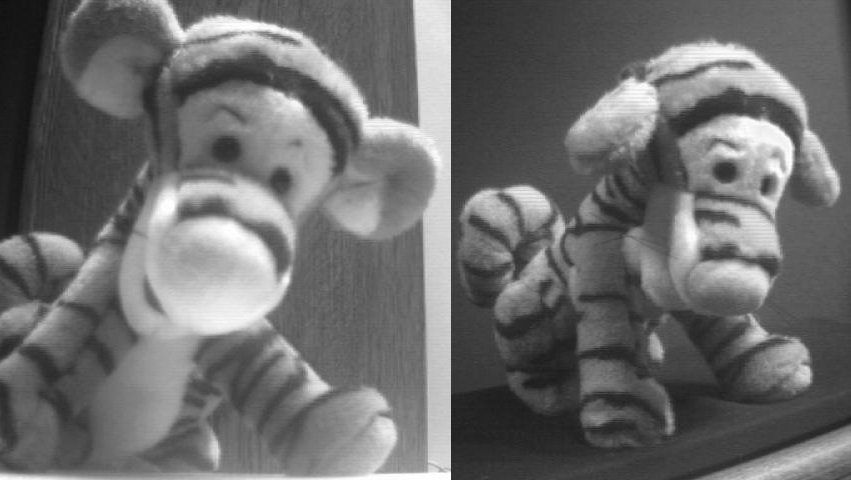
\includegraphics[width=75mm]{figuras/tigger-mit.png}
  \end{center}
  \caption{Brinquedo que responde as emoções das crianças \cite{kirsch1999affective}.}
  \label{fig:tigger-mit}
\end{figure}

O projeto \emph{The Affective Tigger: a reactive expressive toy} de
\citet{kirsch1999affective} é um brinquedo capaz de reconhecer e reagir às
emoções exibidas pelas crianças. Por exemplo, quando a criança encontra-se
feliz, o boneco expressa felicidade (ver Figura~\ref{fig:tigger-mit}). Ao todo
existem 5 estados emocionais: muito feliz, feliz, neutro, triste e muito
triste. Todos, com exceção do neutro, possuem alguma síntese vocal como um
rosnado (tristeza) ou uma risada (muito feliz). Assim, esse brinquedo, por ser
considerado um ser robótico que reage à criança com seus próprios estados
emocionais, fica enquadrado na segunda área.  Portanto, o desenvolvimento
desse brinquedo serviu para aprimorar os seres robóticos.

O projeto AIDA\footnote{Mais detalhes, ver http://senseable.mit.edu/aida} (do
inglês \emph{Affective Intelligent Driving Agent}) pode ser entendido como
enquadrado na área de IHC, pois o interesse é entender o estado afetivo da
pessoa dirigindo. Além disso, interessa-se em ter um relacionamento com o
usuário sugerindo alterações nas rotas baseado na rotina aprendida depois de
um mês de aprendizado.  A pesquisa relatada em \citet{dias-agents} visou
melhorar a simulação de agentes através do uso da emoção guiando o processo
deliberativo e melhorar o entendimento e gerência das emoções.  O presente
trabalho se enquadra na área de síntese de emoção, pois o interesse é em
entender o estado emocional e como ele pode afetar o comportamento de um
personagem.

\section{Modelo Psicológico de Emoção}

Segundo \citet{scherer2000tnoe}, na psicologia há diferentes modelos para
tentar mapear a afetividade: dimensionais, discretos, baseados em significados
e componentes. Os modelos dimensionais procuram estabelecer eixos de classes
de emoções e formas de se mover por esses.  Enquanto os modelos discretos
visam descrever um conjunto básico de emoções ou, ainda, um sistema adaptativo
que evolua a partir de um determinado ponto.  Os modelos baseados em
significados constroem estruturas semânticas e descrevem verbalmente o que
ocorre em determinado sentimento; em outras palavras, preocupa-se com as
situações em que ocasionaram o mesmo. Já os modelos baseados em componentes
entendem que emoções são aprendidas e, sendo assim, estudam o elo entre os
sentimentos e os eventos ou situações que as mesmas acontecem. Esse elo é
montado pela pessoa de diferentes formas.

\citet{Pic98} chama atenção que as emoções sempre foram consideradas um
estigma pela ciência que é fundamentalmente racional com hipóteses testáveis,
argumentos lógicos e experimentos repetitivos.  Entretanto, estudos
neurológicos recentes \cite{ledoux1998emotional,damasio2004erro} mostram a
importância das emoções na tomada de decisão.  \citet{damasio2004erro}
diferencia emoção de sentimento; para ele emoção é um estado físico do corpo e
sentimento é a percepção da mudança desse estado corporal.

\begin{figure*}
  \centering
    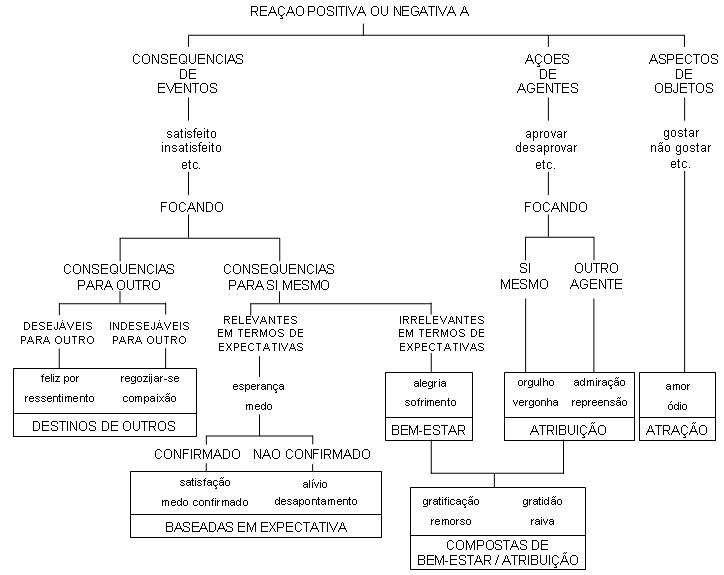
\includegraphics[width=150mm]{figuras/pontarolo_occ.png}
  \caption{Modelo OCC adaptado de \cite{pontarolo2008modelagem}.}
  \label{fig:occ_model_original}
\end{figure*}

O modelo proposto por \citeauthor*{ortony1988cse} \cite{ortony1988cse},
conhecidos na comunidade de Inteligência Artificial, é chamado de OCC por
causa de seus autores.  Esse modelo é classificado como baseado em
significados por descrever as situações de ocorrências de cada uma de suas 22
emoções.  Essas emoções são divididas em formas de se perceber o mundo a sua
volta: Eventos (importantes para alguma meta), Agentes (incluindo a si mesmo)
e Objetos (atração ou repulsa). Assim sendo, essas maneiras de se perceber o
mundo refletem diferentes jeitos de se analisar as situações que podem ser
relativas aos objetivos, valores morais ou gostos da pessoa.

A Figura~\ref{fig:occ_model_original} resume o modelo OCC e mostra as
percepções possíveis de um indivíduo.  Partindo da direita para esquerda, o
ramo mais básico, Aspectos de Objetos, é ativado quando se avalia o gosto de
alguém para algum objeto (inanimado ou não), por exemplo, alguém gostar de
rosas vermelhas.  No seguinte, Ações de agentes, o julgamento das ações
exercidas por outro indivíduo é realizado baseado nos valores morais da pessoa
que está julgando.  Sendo assim, por exemplo, reprovar a atitude de um colega
que ``colou'' na prova. O último da árvore, mais a esquerda, é o de evento que
representa as coisas que aconteceram (e foram consideradas importantes),
acontecem e acontecerão (objetivos almejados). Esses são avaliados segundo as
suas consequências para o alcance ou impedimento dos objetivos de uma pessoa.
Por exemplo, preciso ir bem no concurso para ficar satisfeito porque esse
evento me permitirá alcançar minha meta de ser contratado.

Ainda segundo o modelo OCC, as emoções possuem intensidades. Entretanto, há
distinção entre a valência da emoção e a valência do sentimento. No modelo, um
indivíduo só possui o sentimento quando a intensidade da emoção ultrapassar um
determinado limite.  Essa intensidade é obtida por uma função matemática que
utiliza variáveis de dois tipos: local, que influencia as emoções em um ramo
específico; e global, que influencia todas as emoções do indivíduo.  Um
exemplo de variável local é o desejo, enquanto que um exemplo de variável
global é o senso de realidade.

\section{Ontologias}

\todo{reescrita} Desde Aristóteles, de acordo com \citet{wks2008towards},
começa o estudo das coisas existentes no mundo e a natureza desse existência,
um ramo da filosofia conhecido com ontologia.  Atualmente, na ciência da
computação, ontologias são vistas como um vocabulário de entendimento comum e
compartilhado de um domínio que pode ser utilizada para comunicação entre
pessoas e aplicações distribuídas e heterogêneas.  \citet{ontoly2004Approach}
definem ontologia como uma representação de conhecimento utilizada para
capturar conhecimento e informação sobre determinado assunto, geralmente
estruturado de forma similar a uma rede semântica. Sendo assim, uma ontologia
consiste de um diagrama composto de nodos e arcos que estabelecem uma
fundamentação semântica que permite melhorar a descoberta, interoperabilidade
e reuso do conhecimento.

Logo, o conhecimento pode ser usado de maneiras diferentes e não serve somente
para conter informações em categorias, mas também serve como um tipo de
``banco de dados'' onde instâncias são armazenadas e recuperadas.  O tipo ou
classe da informação possui propriedades que diferem da sua instância. Essa
diferença fica clara quando é feita a comparação da ontologia com uma base de
dados, onde as classes de informações definidas criam as tabelas e as
instâncias povoam os dados nas tabelas.

Na área da computação, ontologias ganharam maior importância com a Web
Semântica permitindo que o conhecimento da página seja facilmente obtido sem
um processamento pesado.  A W3C, orgão internacional que regulamenta padrões
utilizados na Web, regulamentou diversos padrões baseados em \emph{XML} para
ontologias.  A linguagem que será utilizada no presente trabalho será a
OWL\footnote{A sigla vem de ``\emph{Ontology Web Language}''.} e esta fora do
escopo desse artigo aborda-lá em detalhes \footnote{Para mais detalhes, veja
\url{http://www.w3.org/standards/semanticweb/ontology}.}.

\section{Ontologias afetivas}
...

\section{Ontologias de Humanos Virtuais}
...

\section{Trabalhos Relacionados}

O comportamento emotivo do personagem tem um papel importante para se ter a
ilusão de vida conforme afirmou \citet{bates1994role}. Esse trabalho utiliza o
modelo OCC para melhorar a credibilidade dos agentes e cada uma das emoções
pode ser ligada a um comportamento. No exemplo dado anteriormente, um agente
pode ligar o medo a um comportamento agressivo enquanto outro liga essa mesma
emoção de medo a um comportamento de estado alarmado.

\citet{GraCli98} criaram um mecanismo evolucionário utilizando redes neurais
com uma base química para guiar o comportamento do ator. Os atores simulados
podem envelhecer, aprender e, inclusive, se reproduzir (aqui são utilizados
algoritmos genéticos).  Por exemplo, o personagem pode aprender algumas
palavras básicas e demostrar que esta envelhecendo por meio da mudança da cor
de seus cabelos dando uma certa ilusão de vida.

Conforme já dito, as emoções podem melhorar a credibilidade dos seres
virtuais.  \citet{zhang2009emotional} desenvolveram uma aplicação com a
finalidade de demostrar esse conceito. O planejamento das ações a serem
executadas pelo personagem é afetado pelos valores das emoções sendo
experimentadas.

Todos os trabalhos apresentados até aqui, utilizaram as emoções para aumentar
a representação ou expressividade de um ator. Entretanto,
\citet{neto2010construction} tentam estudar o impacto da emoção na decisão dos
agentes.  Assim, para isso ser possível, foi necessário alterar a forma de
planejamento das decisões, além de como recuperar os dados da sua memória.  A
modificação no acesso a memória permite o ``esquecimento'' de determinadas
crenças quando o estado emocional for diferente daquele guardado junto da
memória a ser recuperada. Essa característica torna o planejamento do agente e
as atitudes dos personagens mais realísticas.

\citet{benta2007ontology} e \citet{wks2008towards} descrevem modelos afetivos
através de ontologias. No primeiro trabalho, uma ontologia foi criada
descrevendo emoções primárias e secundárias. O primeiro tipo de emoção exige
menos processamento cognitivo que o segundo. Além disso, o modelo descreve ao
todo 11 emoções sendo 7 dessas consideradas primárias.


\chapter{Trabalho Desenvolvido} \label{chap-desenvolvimentoWS}

O trabalho desenvolvido visa permitir que a plataforma Jason possa
ter tanto ambiente quanto agentes implementados em outras linguagens. Assim, a
plataforma Jason pode ser considerada uma arquitetura totalmente aberta, dado
que, até o raciocínio dos agentes poderia ser feito fora da plataforma.
A explicação de qual dos protocolos foi escolhido debatendo os critérios
utilizados e a estrutura de métodos necessários no servidor será explicado na
seção \ref{sec-WSS}. O cliente desses métodos fica localizado dentro da
plataforma Jason e os detalhes da implementação podem ser vistos na seção
\ref{sec-WSC}.

\section{Servidor de Serviços Web} \label{sec-WSS}

No capítulo \ref{chap-introducao} foi comentado que tanto SOAP quanto XML-RPC são
mecanismos comuns para o conjunto de linguagens escolhidos, pois não importa
qual deles se escolha haverá sempre pelo menos uma biblioteca para uso. Assim,
o critério decisivo utilizado para decidir foi a simplicidade, visto que
isso reflete nas mensagens e na curva de aprendizagem. Por exemplo,
desconsiderando os dados entregues nas mensagens trocadas tem-se que o SOAP
envia 472 bytes e o XML-RPC 173 bytes. Além disso, a curva de aprendizagem
do XML-RPC é menor pois há quase seis vezes menos tipos de dados que o
padrão SOAP.

\begin{figure}[h]
               \begin{center}
               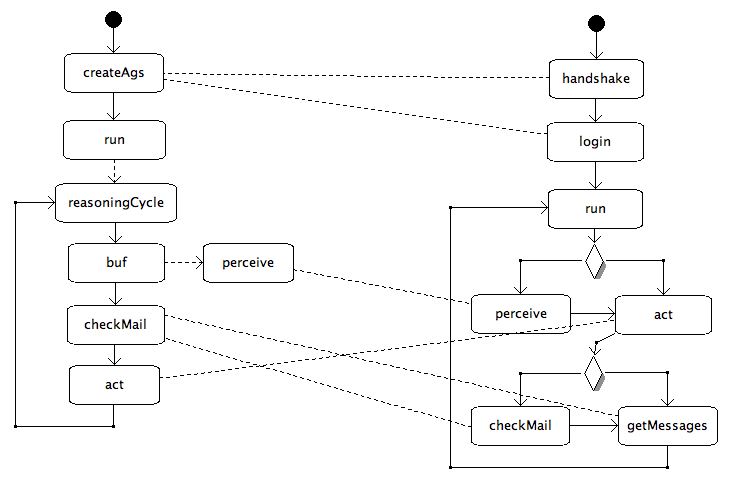
\includegraphics[width=104mm]{figuras/implXR-ag-compare-cycle.png}
                \end{center}
                \caption{Diagrama relacionando o ciclo do agente Jason (esquerda) com os métodos à serem implementados em serviços (direita).}
                \label{fig-uml-ag-cycle}
\end{figure}

Com o protocolo a ser utilizado definido, tudo que resta é definir como os
agentes e o ambiente podem ser implementados utilizando WS. Um servidor sempre
representa uma coleção de entidades do seu tipo determinado. No caso do
ambiente deve-se lembrar que todos os métodos influenciarão um único ambiente
compartilhado por diversos agentes.

\begin{table}
	\caption{Definição dos métodos obrigatórios no servidor de agentes.}
	\label{table-server-agents}
	\begin{center}
	\begin{tabular}{|p{34mm}|p{50mm}|p{50mm}|} % 140mm
		\hline
		Método & Parâmetros & Descrição \\ \hline
		handshake & Desafio (String). & Resolve um desafio proposto. \\ \hline
		login & Nome do agente (String). & Devolve um identificador (ID) numérico do agente. \\ \hline
		logout & ID (Numero) & Libera o ID associado com um determinado agente. \\ \hline
		perceive & ID (Numero) e Percepções (Array) & Associa um conjunto de percepções e retorna a ação do agente especificado.\\ \hline
		act & ID (Numero) e Esvaziar percepções (Boolean) & Esvazia as percepções do agente e retorna sua ação. \\ \hline
		checkMail & ID (Numero) e Mensagens (Array) & Entrega as mensagens
novas e retorna as mensagens à serem enviadas aos outros agentes.\\ \hline
		getMessages & ID (Numero) & Retorna todas as mensagens à serem enviadas aos outros. \\ \hline
	\end{tabular}
	\end{center}
\end{table}

Na Tabela~\ref{table-server-agents} há as definições sobre os métodos
obrigatórios a serem implementados no lado do servidor. Esses métodos são
chamados pela plataforma Jason em momentos específicos para operar o agente.
Os métodos \emph{handshake} e \emph{login} são chamados durante a criação do
agente na inicialização da plataforma Jason. O primeiro método recebe um
desafio (uma string qualquer) e deve responder o desafio da forma esperada.
Desse modo, a plataforma Jason sabe que o WSS sendo utilizado tem o mínimo de
confiabilidade exigido. O segundo método, \emph{login}, serve para associar um
identificador único com determinado agente. Esse identificador é utilizado nas
chamadas seguintes da plataforma Jason. Ao término da plataforma Jason a
função \emph{logout} é chamada para liberar o identificador único
criado.%\dev{hoje nao ha protecao aqui e nao tera}

Todo agente se comunica com outros agentes em algum nível, seja ela de forma
direta (recebendo uma mensagem de outro) ou indireta (alterações de percepções
do ambiente). Para a comunicação direta existir entre agentes fora da
plataforma Jason, existem os métodos \emph{checkMail} e \emph{getMessages}. O
método \emph{checkMail} entrega as mensagens novas para o agente e, ao fim,
chama \emph{getMessages} para devolver todas as mensagens que o agente deseja
enviar para os demais agentes. Note que, se o agente não tiver novas mensagens
à serem recebidas, a plataforma pode chamar de maneira direta a função para
consultar as mensagens à serem enviadas. Esse comportamento é observado na
Figura~\ref{fig-uml-ag-cycle}.

Quanto a forma de comunicação indireta, os agentes percebem modificações no
mundo através de ``sensores'' que refletem as percepções que o agente tem
sobre as coisas no ambiente. De forma análoga às mensagens, as percepções são
alteradas pelo método \emph{perceive}. Esse método serve para cadastrar o
estado atual conhecido do ambiente e tem como retorno uma ação que deve ser
executada no ambiente através do método \emph{act}. A plataforma Jason decide
chamar \emph{act} ao invês de \emph{perceive} quando não houver alterações nos
sensores do agente ou quando não há percepção de nenhum dos sensores (conjunto
vazio).

Na Tabela~\ref{table-server-environment} tem-se a descrição dos métodos
mandatórios para implementação de um WSS como ambiente. Esses métodos lidam em
grande parte com percepções que serão explicados mais adiante. Quando, na
inicialização da plataforma, o agente precisa de informações dos seus
``sensores'' é feita a chamada para o método \emph{handshake}. Ele trabalha da
mesma maneira que o WSS do agente. As funções que adicionam
(\emph{addPercept}), removem (\emph{removePercept}) ou
esvaziam (\emph{clearPercepts}) o conjunto de percepções são aos pares para
deixar claro quando opera no conjunto comum ou específico (são as mesmas
funções, mas terminadas com a palavra Local).

\begin{table}
	\caption{Definição dos métodos obrigatórios no servidor do ambiente.}
	\label{table-server-environment}
	\begin{center}
	\begin{tabular}{|p{34mm}|p{50mm}|p{50mm}|} % 140mm
		\hline
		Método & Parâmetros & Descrição \\ \hline
		handshake & Desafio (String). & Resolve um desafio proposto. \\ \hline
		addPercept & Percepção & Insere uma percepção para todos os agentes.\\ \hline
		addPerceptLocal & Nome do agente (String) e Percepção. & Insere uma percepção para um agente específico. \\ \hline
		clearPercepts & Sem parâmetros. & Apaga as percepções comuns à todos os agentes.\\ \hline
		clearPerceptsLocal & Nome do agente (String). & Apaga as percepções específicas de um agente.\\ \hline
		havePercepts & Nome do agente (String). & Há ou não percepções novas. \\ \hline
		getPercepts &  Nome do agente (String) e envio atualizado (Boolean). & Retorna todas as percepções do agente. \\ \hline
		removePercept & Percepção. & Retira uma percepção comum de todos os agentes. \\ \hline
		removePerceptLocal & Nome do agente (String) e Percepção. & Retira uma percepção que é específica de um agente. \\ \hline
		performAction & Nome do agente (String) e Ação. & O agente executa a ação especificada. \\ \hline
	\end{tabular}
	\end{center}
\end{table}

A recuperação das percepções é feita unicamente via chamada ao método
\emph{getPercepts}. Esse método, quando chamado, recebe o agente operando para
conseguir montar o conjunto de percepções do mesmo e se deve considerar
isso como a percepção do ciclo do Jason para computar como atualização. O
conjunto de percepções enviado é o conjunto comum ou global de percepções
unido com o conjunto de percepções locais ou específicas do agente informado.
O método \emph{havePercepts} serve para informar a plataforma que há novas
percepções ou não, assim a mesma sabe quando pegar as percepções.

Durante toda a simulação o agente realiza alguma ação, seja no ambiente ou
não. Essas ações são realizadas utilizando o método \emph{performAction} que
recebe o agente (executor) e a ação (ato) para saber como as percepções serão
afetadas. A ação recebida utiliza a estrutura de uma percepção. Assim, a
percepção é uma tupla com três elementos: (i) operador, serve como nome da
percepção e tenta dar ideia de qual a finalidade da mesma; (ii) termos, lista
com a finalidade de permitir a parametrização da percepção; (iii) anotações,
lista de percepções referentes a mesma. Logo, a percepção de um agente que
jey é um animal com 55\% de chance de ser um cachorro e 40\% de ser um gato
pode ser expressa da seguinte forma:
``(animal, [jey], [(cachorro, [0.55], []), (gato, [0.40], [])])''.

Cabe salientar ainda que ambas implementações são independentes, isto é, tanto
o ambiente pode ser usado sem a implementação dos agentes quanto os agentes
podem ser usados sem o ambiente. Essa independência permite que os
agentes sejam utilizados com outros agentes da plataforma. Além disso, todo
WSS deve ser desenvolvido com finalidade específica para uma dada simulação.


\section{Cliente de Serviços Web} \label{sec-WSC}

O cliente do WSS fica localizado na plataforma Jason. A
implementação atual estende tanto a classe da arquitetura do agente,
\emph{AgArch}, quanto a classe de ambiente, \emph{Environment}, para
personalizar os comportamentos necessários no uso da plataforma. A
Figura~\ref{fig-uml-ag} demostra a implementação para o agente.

O agente é um cliente de WS e a interface construída para
acessar o servidor implementado. A classe \emph{Perceive} possui a
responsabilidade de traduzir uma tupla de percepção \footnote{Explicada na
seção \ref{sec-WSS}.} do e para o formato da plataforma. Já a classe
\emph{AgentClient} tem a responsabilidade de ser o único acesso ao WSS.
O uso dessa classe é feito pela de arquitetura do agente que sabe o momento
que ele precisa de uma coisa ou de outra.

\begin{figure}[h]
               \begin{center}
               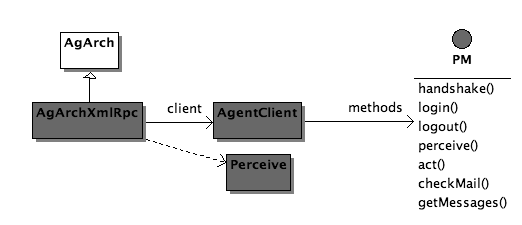
\includegraphics[width=100mm]{figuras/implXR-ag.png}
                \end{center}
                \caption{Diagrama da arquitetura do agente desenvolvido.}
                \label{fig-uml-ag}
\end{figure}

As mensagens de comunicação trocadas entre os agentes para uma comunicação
direta são tuplas com o seguinte formato: (i) identificador único da
mensagem; (ii) quem esta emitindo a mensagem, não é necessário preenche-lo;
(iii) tipo da mensagem sendo enviada, de preferência aos formatos
existentes do Jason; (iv) a quem se destina a mensagem sendo enviada; (v)
mensagem sendo enviada. Desta forma, quando se deseja dizer para um agente
(beltrano) que o disco esta gravado então a seguinte mensagem será enviada:
``<id42,,tell,beltrano,disco(gravado)>''. As crenças dos agentes,
entretanto, podem ser pensadas de duas formas: (i) o agente é responsável por
manter internamente suas crenças; (ii) o agente guarda suas crenças junto das
percepções utilizando as ações do ambiente.

Dadas essas duas opções, foi trabalhado com a segunda, que guarda as
percepções e crenças dos agentes no ambiente e parece ser um modelo mais
próximo do que existe hoje na plataforma Jason. Dessa forma, daqui por diante,
quando for mencionado, o dado de percepção este fará
alusão tanto a elementos percebidos do ambiente quanto crenças, conclusões ou
desejos feitos pelo agente. Assim, o ambiente é
responsável por armazenar as percepções dos agentes e por conhecer como as
ações dos agentes devem ser desempenhadas. Tanto o ambiente quanto o agente
possuem uma estrutura de classes semelhantes. Essa semelhança tem como
vantagem o ganho de velocidade quando, por ventura, for necessária alguma
modificação no futuro.

Dessa forma, o desenvolvimento do lado do ambiente seguiu um modelo parecido
com o do agente, conforme pode ser visto na Figura~\ref{fig-uml-env}. Essa
figura explica que o ambiente desenvolvido (classe \emph{EnvXmlRpc})
especializa o ambiente da plataforma (classe \emph{Environment}) para se
responsabilizar por quando ir no servidor. A classe \emph{Perceive} tem a
responsabilidade de traduzir as tuplas recebidas de e para o formato da
plataforma, conforme já explicado. A responsabilidade da classe
\emph{EnvironmentClient} é de ser o único meio de acessar o servidor externo.

Além disso, as interfaces servem para padronizar o acesso externo realizado.
Essa escolha pelas interfaces foi feita por dois motivos. O primeiro
foi deixar isolado os métodos que o servidor precisa responder.
Enquanto, o segundo foi tirar vantagem da técnica de reflexibilidade
que permite a construção de métodos que servem de \emph{proxy}. A
implementação do cliente feita na plataforma Jason pode ser visualizada no
Anexo~\ref{anexo-jason}.

\begin{figure}
               \begin{center}
               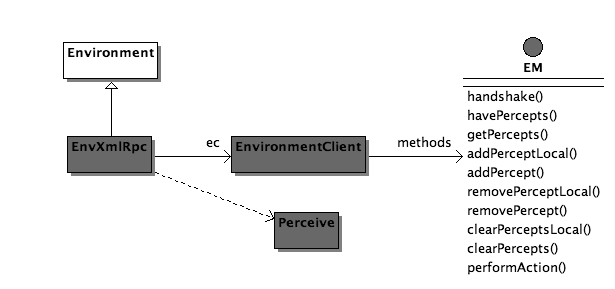
\includegraphics[width=100mm]{figuras/implXR-env.png}
                \end{center}
                \caption{Diagrama do ambiente desenvolvido.}
                \label{fig-uml-env}
\end{figure}


\chapter{Exemplo de Uso} \label{chap-casoWS}

O presente capítulo apresenta dois exemplos desenvolvidos. Na
seção \ref{casoWS-room} se apresenta o exemplo \emph{room} adaptado para
executar dois agentes (\emph{porter} e \emph{paranoid}) na linguagem Python.
Já o seguinte apresenta o exemplo
\emph{game of life}, adaptado para ter o ambiente desenvolvido em Haskell. Os
agentes em Python estão na seção \ref{casoWS-gol}.

\section{Exemplo \emph{Room}} \label{casoWS-room}

O exemplo \emph{Room} foi adaptado para executar dois agentes de maneira
externa à plataforma Jason. Assim, a Listagem~\ref{lst-roomMas2j} (pg.
\pageref{lst-roomMas2j}) deve ficar conforme a Listagem~\ref{lst-roomXR}.
Fora isso, os dois programas que implementam o servidor de agentes do
\emph{porter} e do \emph{paranoid} devem ser disparados antes da plataforma
Jason iniciar a simulação. A implementação desses pode ser vista
no Anexo~\ref{anexo-room}.

\lstset{linewidth=100mm}
\begin{center}
    \begin{minipage}{100mm}
	\begin{lstlisting}[frame=trbl, caption=Arquivo de projeto do Jason adaptado., label=lst-roomXR]
// Isso eh um comentario
MAS room {
  infrastructure: Centralised
  environment: RoomEnv
  executionControl: jason.control.ExecutionControl
  agents:
    porter
    [url="http://localhost:8080"]
    agentArchClass maro.architecture.AgArchXmlRpc
    ;
    claustrophobe
    ;
    paranoid
    [url="http://localhost:8081"]
    agentArchClass maro.architecture.AgArchXmlRpc
    ;
}
	\end{lstlisting}
    \end{minipage}
\end{center}

A Listagem~\ref{lst-roomXR} define uma simulação na plataforma Jason com três
agentes heterogêneos. O primeiro chamado \emph{porter} encontra-se localizado
em um WSS definido pela url ``http://localhost:8080'' que define o
servidor sendo a máquina local na porta 8080. Nessa url poderia ser colocado
lugares diferentes sem nenhum problema e a porta poderia ser omitida quando a
mesma for a 80. O segundo agente nomeado \emph{claustrophobe} é um agente
Jason e o último agente é outro WSS localizado na porta 8081.

A implementação dos agentes em Jason podem ser consultadas na
Listagem~\ref{lst-agente} (página~\pageref{lst-agente}). O agente \emph{porter}
como pode ser visto, deve trancar a porta quando receber do agente
\emph{paranoid} a meta \emph{locked} e deve destrancar a porta quando receber
do agente \emph{claustrophobe} a meta $\sim$\emph{locked}. De acordo com a
Figura~\ref{fig-uml-ag} (pg \pageref{fig-uml-ag}), há 7 métodos que o servidor
necessita implementar. Os métodos \emph{handshake}, \emph{login} e
\emph{logout} não serão comentados aqui.

\lstset{linewidth=130mm}
\begin{center}
    \begin{minipage}{140mm}
	\begin{lstlisting}[frame=trbl, caption=Método de percepção e ação do agente \emph{porter}., label=lst-roomWS-perceive]
def perceive(id, percepts):
	data = agentL[id]
	agentL[id] = (data[0], percepts, data[2])
	return act(id, False)

def act(id, eraseAll):
	if eraseAll:
		data = agentL[id]
		agentL[id] = (data[0], [], data[2])
	data = agentL[id]
	if len(data[2]) >= 1:
		ret = exclusion_act(data[1], data[2][0])
		if len(ret) > 0:
			agentL[id] = (data[0], data[1], data[2][1:])
		return ret
	return ""

def exclusion_act(perceptions, message_received):
	M = { "~locked(door)":"locked(door)", "locked(door)":"~locked(door)" }
	P = { "~locked":"lock", "locked":"unlock" }
	test = M[ message_received[4] ][:-1].split('(')
	for p in perceptions:
		functor = p[0]
		terms = p[1]
		annots = p[2]
		if functor == test[0] and terms[0] == test[1]:
			return P[functor]
	return ""
	\end{lstlisting}
    \end{minipage}
\end{center}

Na Listagem~\ref{lst-roomWS-perceive} tem-se a implementação de dois dos
métodos essenciais. O primeiro (\emph{perceive}) recebe o identificador do
agente criado na inicialização e a nova lista de percepções e usa esses
dados para atualizar a tupla que contêm, respectivamente, o nome do agente, as
percepções e as mensagens recebidas. Agora, o método \emph{act} deve retornar
a ação que o agente \emph{porter} fará no momento e, para isso, recebe o
identificador do agente e um valor lógico que indica se as percepções devem
ser apagadas ou não. Assim, é possível chamar esse método sem passar por
\emph{perceive} quando o grupo de novas percepções for o grupo vazio. Portanto, a
primeira atividade dessa função é verificar esse valor e limpar as percepções
caso seja necessário. Após, o uso verifica se há mensagens, havendo chama
uma função auxiliar para definir se há ou não ação a realizar e consome a
mensagem.

\lstset{linewidth=130mm}
\begin{center}
    \begin{minipage}{140mm}
	\begin{lstlisting}[frame=trbl, caption=Métodos relacionados com a comunicação do agente \emph{porter}., label=lst-roomWS-messages]
def receiveMessages(id, messages):
	data = agentL[id]
	msgL = []
	for msg in messages:
		m = msg[1:-1].split(',')
		if m[1] == "claustrophobe" and m[4] == "~locked(door)":
			msgL.append(m);
		elif m[1] == "paranoid" and m[4] == "locked(door)":
			msgL.append(m);
	agentL[id] = (data[0], data[1], msgL)
	return sendMessages(id)

def sendMessages(id):
	return []
	\end{lstlisting}
    \end{minipage}
\end{center}

O agente que origina à mensagem é testado no momento do recebimento
da mensagem, onde o agente pode descarta-la ou guarda-la.
Esse comportamento pode ser observado na Listagem~\ref{lst-roomWS-messages}.
Nela os métodos \emph{checkMail} e \emph{getMessages} mapeiam,
respectivamente, para \emph{receiveMessages} e \emph{sendMessages}. O método
de recebimento de mensagens, \emph{receiveMessages}, sabe como parsear a tupla
que veio (linha 5) e somente cadastra as mensagens relevantes para desempenhar
as mesmas ações do código Jason. Dessa forma, ele só considera as mensagens
relevantes que para o agente \emph{paranoid} é um pedido de trancamento
e para o agente \emph{claustrophobe} é um pedido de destrancamento da porta.
O agente \emph{porter} não envia nenhum tipo de mensagens para
outros agentes, assim a implementação do \emph{getMessages} mapeado para
\emph{sendMessages} na implentação retorna um conjunto vazio representando que
não deseja enviar mensagens.

\lstset{linewidth=130mm}
\begin{center}
    \begin{minipage}{140mm}
	\begin{lstlisting}[frame=trbl, caption=Métodos do agente \emph{paranoid}., label=lst-roomWS-paranoid]
def act2(id, eraseAll):
	if eraseAll:
		data = agentL[id]
		agentL[id] = (data[0], [], data[2])
	data = agentL[id]
	if len(data[1]) > 0:
		sendMessage = exclusion_act(data[1])
		if len(sendMessage) > 0:
			data[2].append(sendMessage)
			agentL[id] = (data[0], data[1], data[2])
	return ""

def exclusion_act(perceptions):
	p = perceptions[0]
	functor = p[0]
	terms = p[1]
	annots = p[2]
	if functor == "~locked" and terms[0] == "door":
		try:
			msgId = agentL["msgId"]
		except KeyError:
			msgId = 0
		agentL["msgId"] = msgId + 1
		return "<mprpc%02d,,achieve,porter,locked(door)>" % msgId
	return ""

def sendMessages(id):
	data = agentL[id]
	ret = []
	if len(data[2]) > 0:
		ret = data[2]
		agentL[id] = (data[0], data[1], [])
	return ret
	\end{lstlisting}
    \end{minipage}
\end{center}

No agente \emph{paranoid} a situação se altera um pouco, a função de percepção
(\emph{perceive}), ação (\emph{act}) e recebimento de mensagens
(\emph{checkMail}) não são mostrados na Listagem~\ref{lst-roomWS-paranoid}.
O método de percepção é igual ao mostrado
anteriormente, porém ele passa a chamar \emph{act2} ao invés de \emph{act}.
Já no método \emph{act}, o método \emph{act2} só é chamado quando
precisa limpar todas as crenças. O método \emph{checkMail}
simplesmente realiza a chamada a função \emph{getMessages} (mapeada na
implementação para \emph{sendMessages}) para enviar para a plataforma Jason as
mensagens desejadas.

A presente implementação considera uma mensagem como uma string. Essa string
tem o seguinte formato: ``<id, emissor, tipo, vitima, mensagem>''. Esses dados
são usados para construir uma tupla com 5 elementos, conforme já explicado na
seção \ref{sec-WSC}. Essa string é construída na função interna
\emph{exclusion\_act}, chamada somente quando há percepções, e
guardada para ser enviada depois pela função \emph{getMessages}. Essa função
retorna as mensagens que o agente deseja enviar e limpa o campo de
mensagens à serem enviadas.


\section{Exemplo \emph{Game of Life}} \label{casoWS-gol}

O presente exemplo tem como foco apresentar uma implementação do
ambiente como WS. O serviço segue a interface apresentada na
Figura~\ref{fig-uml-env} presente na página~\pageref{fig-uml-env}, onde
existem 10 métodos.
%
O presente foi organizado em um diretório e um arquivo \emph{Python}. No arquivo
\emph{Python} tem-se a implementação do raciocínio dos agentes e no diretório
tem-se a implementação do ambiente. O ambiente é tanto a implementação da API
pública em WS quanto a interface que o usuário pode interagir (que na versão
Jason existia).

\lstset{linewidth=130mm}
\begin{center}
    \begin{minipage}{140mm}
	\begin{lstlisting}[frame=trbl, caption=Arquivo de projeto do \emph{Game-of-Life}., label=lst-gol]
MAS game_of_life {
  infrastructure: Centralised(pool,2)
  environment: maro.Environment.EnvXmlRpc("http://localhost:8079")
  executionControl: jason.control.ExecutionControl

  agents:
    cell
    [url="http://localhost:8080/RPC2"]
    agentArchClass maro.architecture.AgArchXmlRpc
    #3600 // matrix 60x60
    ;
}
	\end{lstlisting}
    \end{minipage}
\end{center}

A Listagem~\ref{lst-gol} mostra o arquivo de projeto adaptado. Na URL a parte
com ``RPC2'' poderia ser omitida deixando somente o endereço com a porta. O
ambiente recebe a URL da maneira como demostrada. A infraestrutura utilizada é
a centralizada, porém é utilizado um conjunto de \emph{threads} que no caso
foi definido no valor 2 (duas \emph{threads}).

\lstset{linewidth=73mm}
\begin{wrapfigure}{l}{83mm}
    \begin{minipage}{73mm}
	\begin{lstlisting}[frame=trbl, caption=Tipos usados pelo ambiente.,label=lst-gol-types]
type Action = Percept
data Percept = Percept {
        functor::String,
        params::[String],
        annots::[Percept]
    } deriving (Show,Eq,Ord)
data TPerception = Perceptions {
        global::[Percept],
        local::[(String, Percept)],
        updated::[String]
    } deriving (Show)
	\end{lstlisting}
    \end{minipage}
\end{wrapfigure}

Antes de mostrar os trechos da implementação da parte do ambiente em
\emph{Haskell} é necessário falar sobre os dois tipos de dados que são usados para
suportar o desenvolvimento. Na Listagem~\ref{lst-gol-types} tem-se os tipos, o
primeiro denominado \emph{Percept} é a tupla de percepções explicada na
seção~\ref{sec-WSS}. Esse tipo de dado também pode ser referenciado como
\emph{Action}. Já o tipo \emph{TPerception} contém, respectivamente,
uma lista de percepções, uma lista com tuplas que mapeam nome do agente para uma
percepção e uma lista de nomes de agentes. Esse tipo serve para guardar
separadamente as percepções globais dos locais e guarda ainda os agentes que
estão atualizados (o cliente já requisitou os dados atuais). Cabe salientar,
ainda, que todas as listas são mantidas ordenadas para facilitar a busca
nas mesmas.

Na Listagem~\ref{lst-gol-arcP} são mostrados os métodos implementados pelo WSS
para adicionar, remover e limpar as percepções locais ou globais.
Esses métodos tratam a lista de
percepções que eles alteram como conjuntos. Dessa forma, não é necessário se
preocupar com percepções repetidas porque elas não vão existir. Além disso,
nas operações de remoção e limpeza é utilizada a
diferença entre dois conjuntos. Essas funções da listagem encontram-se
mapeadas e publicadas por um WS, porém, quando comparadas com a
Tabela~\ref{table-server-environment} (pg \pageref{table-server-environment})
pensa-se que há parâmetros em excesso. Na implementação do método
\emph{addPerceptLocal}, por exemplo, têm-se por parâmetros uma referência ao
tipo interno \emph{TPerceptions}, uma \emph{string} (nome do agente), uma
tupla de percepção e como retorno um booleano encapsulado. Esse protótipo de
função é possível pois quando se realiza o mapeamento das funções publicadas
pelo WS passa-se alguns parâmetros da chamada a priori.
Essa característica é utilizada em quase todas as funções e,
principalmente, na \emph{performAction}. Consulte no Anexo~\ref{anexo-gol} a
função \emph{serving} (pg~\pageref{anexo-gol-endLuccaWS}) para maiores
detalhes.

\lstset{linewidth=140mm}
\begin{center}
    \begin{minipage}{140mm}
	\begin{lstlisting}[frame=trbl, caption=Métodos relativos às percepções.,label=lst-gol-arcP]
addPercept :: IORef(TPerception) -> Percept -> IO Bool
addPercept p perception = do
    (Perceptions gp lp ua) <- readIORef p
    let gp' = insertSet perception gp
    modifyIORef p $ \(Perceptions _ lp _) -> (Perceptions gp' lp [])
    return True

addPerceptLocal :: IORef(TPerception) -> String -> Percept -> IO Bool
addPerceptLocal p name perception = do
    (Perceptions gp lp ua) <- readIORef p
    let lp' = insertSet (name,perception) lp
    modifyIORef p $ \(Perceptions gp _ _) -> (Perceptions gp lp' [])
    return True

removePercept :: IORef(TPerception) -> Percept -> IO Bool
removePercept p perception = do
    (Perceptions gp lp ua) <- readIORef p
    let gp' = gp `minus` [perception]
    modifyIORef p $ \(Perceptions _ lp _) -> (Perceptions gp' lp [])
    return True

removePerceptLocal :: IORef(TPerception) -> String -> Percept -> IO Bool
removePerceptLocal p name perception = do
    (Perceptions gp lp ua) <- readIORef p
    let lp' = lp `minus` [(name,perception)]
    modifyIORef p $ \(Perceptions gp _ _) -> (Perceptions gp lp' [])
    return True

clearPercepts :: IORef(TPerception) -> IO Bool
clearPercepts p = do
    (Perceptions gp lp ua) <- readIORef p
    if (null gp) then
        return True
     else do
        modifyIORef p $ \(Perceptions _ lp _) -> (Perceptions [] lp [])
        return True

clearPerceptsLocal :: IORef(TPerception) -> String -> IO Bool
clearPerceptsLocal p name = do
    (Perceptions gp lp ua) <- readIORef p
    if (null gp) then
        return True
     else do
        let lp' = lp `minus` [(name, perception) | (n, perception) <- lp, n==name]
        modifyIORef p $ \(Perceptions _ lp _) -> (Perceptions [] lp [])
        return True
	\end{lstlisting}
    \end{minipage}
\end{center}

O ambiente é responsável por armazenar todas as percepções que os agentes
possuem, assim ele deve também disponibilizar formas desses dados serem
recuperados. A Listagem~\ref{lst-gol-testP} mostra os dois métodos que são
usados no momento do agente conhecer as suas percepções. A função
\emph{havePercepts} utiliza a lista de agentes atualizados para devolver
verdadeiro quando é necessário ocorrer uma chamada ao método
\emph{getPercepts}. O  método \emph{getPercepts} define as percepções à
serem retornadas na linha 9 da Listagem~\ref{lst-gol-testP} como sendo a
união das percepções globais com o conjunto de percepções locais filtrados
pelo nome do agente.

\begin{center}
    \begin{minipage}{140mm}
	\begin{lstlisting}[frame=trbl, caption=Métodos para recuperar as percepções., label=lst-gol-testP]
havePercepts :: IORef(TPerception) -> String -> IO Bool
havePercepts p name = do
    pp <- readIORef p
    return $ not $ (updated pp) `has` name

getPercepts :: IORef(TPerception) -> String -> Bool -> IO [Percept]
getPercepts p name isUpdate = do
    (Perceptions gp lp ua) <- readIORef p
    let r = union gp [lp' | (n, lp') <- lp, n == name]
    if isUpdate == False then
        return r
     else do
        let ua' = insertSet name ua
        modifyIORef p $ \(Perceptions gp lp _) -> (Perceptions gp lp ua')
        return r
	\end{lstlisting}
    \end{minipage}
\end{center}

A presente implementação do ambiente aceita quatro ações possíveis vindo do
agente Jason. As ações nomeadas são \emph{skip}, \emph{live} e \emph{die}, uma
quarta ação existe e é a ação de ignorar para quando o ambiente não conhece-la não
realizar nenhuma tarefa. Essa seleção é feita baseado no operador da ação
recebida (linha 5 da Listagem~\ref{lst-gol-action}).

\lstset{linewidth=130mm}
\begin{center}
    \begin{minipage}{140mm}
	\begin{lstlisting}[frame=trbl, caption=Método que realiza ações., label=lst-gol-action]
performAction :: IORef(TPerception) -> SyncModel -> GLWidget -> String
     -> Action -> IO Bool
performAction p controller viewer name action =
    let
        actionName = functor action
        actionPars = params action
        actionBy = name
    in
        case actionName of
            "skip"  -> cmdRealize p controller viewer actionBy Nothing
            "live"  -> cmdRealize p controller viewer actionBy (Just True)
            "die"   -> cmdRealize p controller viewer actionBy (Just False)
            _       -> return True -- ignore action
	\end{lstlisting}
    \end{minipage}
\end{center}

Na Listagem~\ref{lst-gol-action}, a chamada a função interna \emph{cmdRealize}
permitiu que fosse abstraído código. Essa é a função que
realiza o trabalho ``sujo'' de atualizar o modelo e solicitar a reexibição da
interface com o usuário. Os únicos parâmetros úteis para a célula são: a
referência as percepções, quem está realizando a ação e que tipo de ação é.
Para representar o tipo de ação é utilizado o tipo \emph{Maybe Bool}. Dessa
forma, as funções \emph{skip}, \emph{live} e \emph{die} são mapeadas,
respectivamente, para não ser um tipo booleano ou ser um tipo booleano valendo
verdadeiro ou ser um tipo booleano valendo falso. Maiores detalhes consulte o
Anexo~\ref{anexo-gol}.


\chapter{Considerações finais}

O presente artigo visa apresentar uma visão do trabalho que está sendo feito
para a construção de um simulador no qual os atores e ambientes interagem.
Entretanto, a ontologia foi omitida porque está ainda sendo aprimorada.  A
idéia apresentada não é nova, porém, o ponto chave é a ontologia permitir aos
agentes raciocinarem sobre suas emoções de forma transparente.  Essa
transparência é útil porque permite ao animador conhecer e, até mesmo,
especificar o personagem com um grau bastante elevado de abstração.
%
Dessa forma, dois agentes com a mesma especificação, ao enfrentarem a mesma
situação, terão o mesmo comportamento quando tiverem vivenciado as mesmas
experiências. Essa experiência inclui as informações adquiridas sobre o
ambiente e sobre os demais atores e não somente os interesses e metas do
mesmo.

O modelo OCC em uso no presente trabalho, foi definido em
\citeyear{ortony1988cse} e possui ao todo 22 emoções especificadas por regras
que demonstram quando a mesma acontece. Entretanto, em nenhum momento da sua
definição foi tratado explicitamente como uma emoção afeta as outras presentes
no personagem.
%
A ferramenta em desenvolvimento tem como interesse a simulação computacional
do comportamento humano e, dessa forma, ela pode ser utilizada de diferentes
maneiras e pode coletar diferentes informações para análises com diversos
propósitos.


%\nocite{*} % Citar todos do arquivo bibtex, mesmo quando nao citado
%\bibliographystyle{abnt-alf} % eh o defauult do abntcite
%\bibliographystyle{plainnat} % para ser usado com o natbib
\bibliography{mestrado}

\appendix

\chapter{Fonte do cliente WS na plataforma Jason} \label{anexo-jason}

\lstset{language=Java}
\lstset{linewidth=140mm}
\lstset{backgroundcolor=}
\lstset{breaklines=true}
\lstset{nolol}

\subsection*{Arquivo referente a interface dos métodos do ambiente: xmlrpc/EM.java}
\lstinputlisting[]{anexos/jason/xmlrpc/EM.java}

\subsection*{Arquivo referente a interface dos métodos dos agentes: xmlrpc/PM.java}
\lstinputlisting[]{anexos/jason/xmlrpc/PM.java}

\subsection*{Arquivo responsável pela serialização dos dados Jason: xmlrpc/Perceive.java}
\lstinputlisting[]{anexos/jason/xmlrpc/Perceive.java}

\subsection*{Arquivo responsável pelo acesso ao agente: xmlrpc/AgentClient.java}
\lstinputlisting[]{anexos/jason/xmlrpc/AgentClient.java}

\subsection*{Arquivo responsável pelo acesso ao ambiente: xmlrpc/EnvironmentClient.java}
\lstinputlisting[]{anexos/jason/xmlrpc/EnvironmentClient.java}

\subsection*{Arquivo referente ao ambiente Jason: Environment/EnvXmlRpc.java}
\lstinputlisting[language=Java]{anexos/jason/Environment/EnvXmlRpc.java}

\subsection*{Arquivo referente à arquitetura do Agente Jason: architecture/AgArchXmlRpc.java}
\lstinputlisting[]{anexos/jason/architecture/AgArchXmlRpc.java}

\subsection*{Arquivo referente ao Raciocinador do Agente Jason: asSemantics/AgXmlRpc.java}
\lstinputlisting[]{anexos/jason/asSemantics/AgXmlRpc.java}

\chapter{Fonte do exemplo \emph{Room}} \label{anexo-room}

\subsection*{Arquivo de construção: bin/build.xml}
\lstinputlisting[language=XML]{anexos/room/bin/build.xml}

\subsection*{Arquivo de projeto: Room.mas2j}
\lstinputlisting[]{anexos/room/Room.mas2j}

\subsection*{Arquivo do ambiente: RoomEnv.java}
\lstinputlisting[]{anexos/room/RoomEnv.java}

\subsection*{Arquivo do agente em ASL: claustrophobe.asl}
\lstinputlisting[]{anexos/room/claustrophobe.asl}

%\subsection*{Arquivo de configuração: logging.properties}
%\lstinputlisting[]{anexos/room/logging.properties}

\subsection*{Arquivo do agente em Python: server-paranoid.py}
\lstinputlisting[language=Python]{anexos/room/server-paranoid.py}

\pagebreak
\subsection*{Arquivo do agente em Python: server-porter.py}
\lstinputlisting[language=Python]{anexos/room/server.py}


\chapter{Fonte do exemplo \emph{Game of Life}} \label{anexo-gol}

\subsection*{Arquivo de construção: bin/build.xml}
\lstinputlisting[language=Java]{anexos/gol/bin/build.xml}

\subsection*{Arquivo de projeto: Game-of-life.mas2j}
\lstinputlisting[]{anexos/gol/game-of-life.mas2j}

\subsection*{Arquivo de agente: server-cell.py}
\lstinputlisting[]{anexos/gol/server.py}

\lstset{language=Haskell}
\subsection*{Arquivo de ambiente: hs/Environment.hs}
\lstinputlisting[]{anexos/gol/hs/Environment.hs}

\subsection*{Arquivo de modelo do ambiente: hs/LuccaModel.hs}
\lstinputlisting[]{anexos/gol/hs/LuccaModel.hs}

\subsection*{Arquivo de dados do ambiente: hs/LuccaData.hs}
\lstinputlisting[]{anexos/gol/hs/LuccaData.hs}

\subsection*{Arquivo do mostrador do ambiente: hs/LuccaDisplay.hs}
\lstinputlisting[]{anexos/gol/hs/LuccaDisplay.hs}

\subsection*{Arquivo do receptor do ambiente: hs/LuccaWS.hs}
\lstinputlisting[]{anexos/gol/hs/LuccaWS.hs}
\label{anexo-gol-endLuccaWS}


\end{document}
